\documentclass{llncs}
%
\usepackage{makeidx}  % allows for indexgeneration
\usepackage[british]{babel}
\usepackage{url}
\usepackage[pdftex,colorlinks=true]{hyperref}
\usepackage{graphicx}
%\fussy


\title{A Model of Reproducibility for CAV}

\author{Tom Crick\inst{1} \and Samin Ishtiaq\inst{2} \and Benjamin A. Hall\inst{3}}

\institute{Department of Computing \& Information Systems\\Cardiff Metropolitan University, UK\\
\email{tcrick@cardiffmet.ac.uk}
\and
Microsoft Research Cambridge, UK\\
\email{samin.ishtiaq@microsoft.com}
\and
MRC Cancer Unit, University of Cambridge, UK\\
\email{bh418@mrc-cu.cam.ac.uk}
}

\raggedbottom
\begin{document}
%
\frontmatter          % for the preliminaries
%
\pagestyle{headings}  % switches on printing of running heads
%\addtocmark{} % additional mark in the TOC

\maketitle

\begin{abstract}
Reliably reproducing published scientific discoveries has been acknowledged as a barrier to 
scientific progress. Even when pubhlished results reflect the authors interpretation perfectly,
novel implementation of published algorithms, and their subsequent benchmarking leaves 
substantial room for error. However, whilst this phenomena has been recognised and documented for some
time, there remains only a small subset of software available to support the specific 
needs of the research community (i.e. beyond generic tools such as git). Here we propose a 
concrete platform for reproducibility, based on a prototype which supports previously published 
work by some of the authors. The aim of this platform is to automate the build, unit testing,
and benchmarking of the BioModelAnalyzer software. We propose this prototype as a future
model for promoting and embedding reproducibility into CAV.

\end{abstract}

\section{Introduction}\label{intro}
The reproducibility of scientific discovery has come into sharp focus over the past few years.
Following a revoltion in the sharing and dissemination of published papers (\emph{Open Access})
and the subsequent discussions relating to the sharing of protocols and materials (\emph{Open
Science}) the ability of a researcher to take published data and reimplement the described
workflow has been under scrutiny~\cite{gent:2013,sandve-et-al:2013}. This has been further supported by wider cultural issues in
scientific community, where irreproducible, and frequently high profile results 
are increasingly being identified and retracted from the literature~\cite{retraction_watch}.
We have previously documented some of the technical and cultural barriers to reproducing 
work across multiple disciplines in the computational sciences, both in terms of the sharing
of algorithms~\cite{crick-et-al_recomp2014} and benchmark sets~\cite{crick-et-al_wssspe2}. 
The impact of irreproducibility is however broadly felt across multiple disciplines, with 
well discussed issues psychology~\cite{chambers-et-al:2014} and others.

Reproducibility has now been explicitly acknowledged as a desirable quality in a number of 
different conferences, including CAV (through the CAV Artefact Evaluation) and TACAS. Some conferences explcitly note that 
the provision of \emph{artefacts} (an accessible tool for reproducing results) is desirable
but does not change the ultimate outcome of the review e.g. OOPSLA. Several biological journals
(e.g. Bioinformatics, PLoS Computational Biology) explicitly require that source code is
made available under an open source license, or through a web interface. 

%Cite: Recomputation Manifesto~\cite{gent:2013}, 10 Simple Rules for Reproducible
%Research~\cite{sandve-et-al:2013}, Stodden~\cite{stodden-et-al:2013},
%changes to dissemination in other fields e.g. psychology~\cite{chambers-et-al:2014}.

% http://2014.splashcon.org/track/splash2014-artifacts#About
From SPLASH: {\emph{OOPSLA Artifacts: The Artifact Evaluation Committee has been formed
to assess how well paper authors prepare artifacts in support of such
future researchers. Roughly, authors of papers who wish to participate
are invited to submit an artifact that supports the conclusions of the
paper. The Artifact Evaluation Committee will read the paper and
explore the artifact to give the authors third-party feedback about
how well the artifact supports the paper and how easy it is, in the
committee’s opinion, for future researchers to use the artifact. This
submission is voluntary and will not influence the final decision
regarding the papers. Papers that go through the Artifact Evaluation
process successfully receive a seal of approval printed on the first
page of the paper in the OOPSLA proceedings.}}

Other examples: ACM TRUST~\cite{fursin+dubach:2014}; using proofs and
Coq e.g. POPL/PLDI/ICFP.

% Q: do we need to define artefact? different from model, etc, also
% domain terminology e.g. CS vs. physics.

However, whilst provision of a single implementation or the current source
code may not be sufficient to reproduce computational discoveries satisfactorily.
As discussed previously, external dependencies may change the behaviour, or 
in the case of an incompatible upgrade, prevent compilation. Other factors include
... These points of failure could be partially addressed by going beyond the sharing
of source code and benchmarks, and sharing complete systems which build code and 
test the software in question. Such a system could be run centrally, independent of 
the researchers, and new papers could be associated with a submission of code and
a set of benchmarks. This would ensure that the code compiles and runs as described,
but would also serve as a repository of artefacts, allowing future researchers,
who are perhaps suffering under a burden of code which does not compile or models
which do not behave, a trusted example of a working implementation.

Here we propose an initial specification for a reproducibilty service. We propose the
requirements of a prototype, a suggested plan for introducing the tool to the community,
and a worked example describing how we would expect the tool to work, based on a previous
CAV paper by the authors. Finally, we highlight key implementation issues relating to
security and general applicability which will need mitigating or solving prior to universal
uptake.

\section{A specification for reproducible computational science}\label{spec}

A service for reproducibility is intended to play three important roles. It should:
\begin{enumerate}
	\item Demonstrate that a piece of code can be compiled, run and behaves as described,
		without manual intervention from the developer.
	\item Store and link specific artefacts and their with different publications
		or other publically accessible datasets.
	\item Allow new benchmarks to be added, by users other than the developer, to 
		widen the testing and identify potential bugs.
\end{enumerate}
 
Furthermore, we feel that such a service must require the minimum developer intervention.
This serves multiple purposes- through automation for example, the service can be enabled to compile 
new code and test new benchmarks trivially. This also forces the developer to make local
workarounds or hacks publically viewable. As such, this requires the developer to make the 
project dependencies clearly available, and enables future changes in the dependencies 
(such as a library update) to be tested automatically too. 

Finally, the service must fit easily into the developers workflow. As noted below~\ref{rollout}
we expect that there will be some costs to the users in terms of the time required
to ensure that the code compiles and runs on the service. To minimise this, the service
needs to connect to standard code repositories, automatically detecting and responding to
new versions of the code and updates to dependencies, running tests for every new code commit.

\begin{figure}[h!]
	\centering
	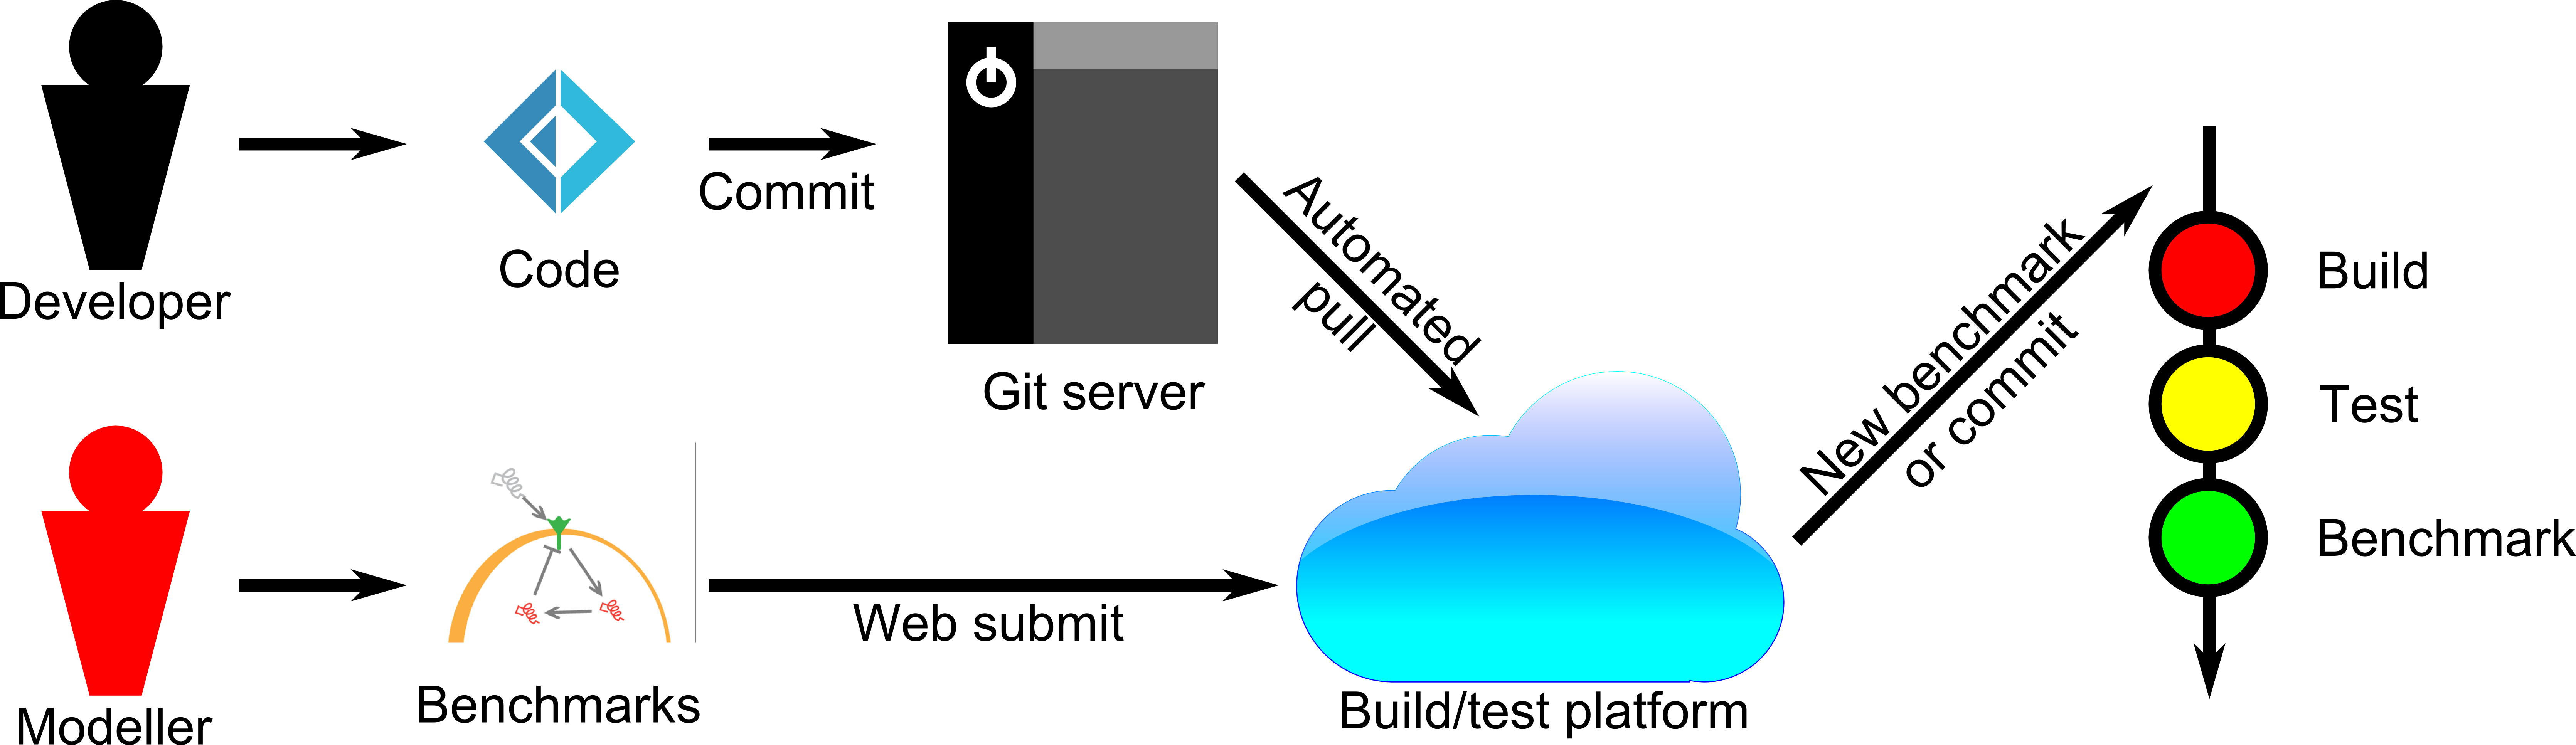
\includegraphics[width=0.9\textwidth]{workflow}
	\caption{Proposed service workflow.}
	\label{schematic}
\end{figure}
	
To address these needs we propose that the service should follow the scheme given in 
figure~\ref{schematic}. Two classes of user are defined; developers, who generate code, 
and modellers, who generate new benchmarks. An individual might in practice play either
or both of these roles; here the roles serve to define ways in which people interact with
the system. A developer writes new code, which is periodically pushed to a repository 
such as github. Through integration with the repository, the server responds to new 
code by undergoing a process of pulling the code from the repository, downloading 
required dependencies, and compiling the code. If this stage fails, the developer is 
informed and the workflow ends. If the code is successfully compiled, two stages of 
testing are performed. The first stage (labelled "test" in figure~\ref{schematic}), involves
running a series of basic tests defined by the developer. This is intended as a sanity check 
to ensure that basic features of the code have not been broken by the updated code, and 
failure to pass these tests is reported and ends the work flow. If this completes succesfully,
the second stage (labelled "benchmark" in figure~\ref{schematic}) a series of models are 
tested for a known property, and the results recorded. These results can then be stored
in a database, with a note of the commit ID, and presented through a web interface for 
future analysis. 

In contrast to the developer role, a modeller supplies benchmarks for a piece of code 
to test. These do not require that the latest version of the code is recompiled, but 
on submission the models are tested and added to the local repository of models for
analysis. After a model is submitted, the model is tested on every new piece of code
pushed to the server and the changes in the behaviour can be noted and linked to 
specific code commits. Whilst the developers role has a transparent value (in 
providing an implementation of an algorithm), the value of the modeller may be less 
immediately clear. The modeller submits a broad range of tests which may highlight
material flaws (i.e. bugs) in the implementation, or the algorithm. More than this
however, the modeller may generate models which identify weaknesses of either an
algorithm or an implementation. One example from the authors experience is the 
series of models with "timed-switches" described in \cite{cook2014}; this is discussed 
in greater depth below in~\ref{example}.

Finally, dependencies for a given implementation need explicit testing. Due to the
highly variable and sometimes complex nature of dependencies, we see this as an
optional part of the workflow, as developers may chose to supply dependencies as
binary files in the code compilation process. For completeness however we note that 
such a system could also respond to updates in external dependencies by triggering 
compilation and testing in the same manner as defined for a new code commit. This 
would aid developers in identifying code breaking changes induced by third parties.


\section{Introducing reproducibility testing to the community}\label{rollout}

Following the proposal of such a system, the question becomes: how do we achieve 
widespread uptake, or even standardisation? Such a service may appear trivial, given the large numbers of tools which
could potentially support the service. There remain however key questions that
can only be answered on implementation. Furthermore, after such a service has been
implemented, how do we ensure it is \emph{useful} and \emph{usable} for researchers.

The key question for different research communities then becomes: how to initialise 
this change? Such a requirement creates a set of new costs to researchers, both in 
terms of time spent ensuring that their tools work on the centralised system (in 
addition to their local implementation), but also potentially in terms of equipment
(in terms of running the system). Such costs may be easier to bear for some groups 
compared to others, especially those with large groups who can more easily distribute 
the tasks, and it is important that the service does not present a barrier to early 
career researchers and those with efficient budgets. This type of cost is not unique 
to reproducibility efforts- it has been estimated (in CACM, a closed but arguably 
affordable journal) that a shift to becoming exclusively open access may lead to a 
ten-fold increase in computer science publication costs~\cite{vardi-cacm-2014}. The
benefits to the community from a cultural change to favour reproducibility are clear
however, and as such we should aim through the software and the roll-out to mitagate 
these costs. Furthermore,
we can reasonably expect the needs of the community to evolve over time, and initial 
implmentations of the platform may require refinement in response to user feedback. As
such, if the community is to move to requiring reproducibility, it seems most reasonable
that this is staggered over a number of years to allow for both of these elements to
develop. We recommend that the tools pass through two testing phases, until eventually
all authors are required to use the service.

Phase 1: Offer the service as an optional extra in the testing phase, allowing users to demonstrate 
the reliability of their code which could be taken into account in the review process.

Phase 2: All authors must use the reproducibility service, but results are not used in the review
process. The results of the test are used to refine the service and pick out any unaddressed issues

Phase 3: All authors are required to use the service, and the results are explicitly used to 
assess reproducibility in the review process.

This plan balances competing needs within the community, and would reduce the activation
energy for uptake by gradually introducing it to authors.

\section{The BioModelAnalyzer as a worked example}\label{example}

{\textbf{IDEA: pick one of Samin's CAV papers (BMA?) and run it through the process
and see what happens.}}

The BioModelAnalyzer is a tool for the development and analysis of a specific 
class of formal models for biology~\cite{benque2012,cook2010,cook2014}. Models 
are built by biologists in a web browser and are explored at present by a combination 
of simulation and model checking. The tool specifically allows users to test for 
model \emph{stability}; that is, a bespoke algorithm proves that for all initial 
states a model always ends in a single fixpoint. We have choosen this example due
to our familiarity with the tool, and to highlight historical examples where a 
reproducibility service would have supported both code development and algorithm
discovery.

Suggested things to discuss here- the proposed benefits of such a service:

Local hacks to publish are not communicated preventing reuse
(specific commands required to compile and publish the code, 
relating to 64- and 32- bit capabilities, were not distributed
and lost when a team member left)
Service would- highlight when a codebase could not be compiled or run

Effects of rounding mechanisms in the algorithm implementation
(swapping floors and rounds broke some things subtly)
Service would- highlight these changes in behaviour clearly

Impact of implementing "biological" intuition in the tool
(changing the default target function of nodes with no inputs, also
breaking things subtly)
Service would- highlight the problems created

Modelling reveals untested issues: range conversion
(no original benchmarks had range conversion- new benchmarks did
and showed unexpected behaviour, including a mismatch between symbolic
and explicit implementations of range conversion)
Service would- allow external users to add new benchmarks, which would make it
easier to catch these issues

Modelling reveals algorithmic weakness: timed switch models 
(a new class of models was discovered which forced the tool to search 
for large cycles explicitly to prove stability)
Service would- allow these new models to have been identified earlier
by highlighting that proofs of stability consistently timed out
Service would- make it easier to prove stability multiple ways (e.g.
through the LTL checker of CAV13)
Service would- show the improvement in speed resulting from the introduction
of the new algorithm

Worked example of how issues could be highlighted and found over time: perhaps
another figure? linking code changes to discoveries could be drawn as a timeline. The 
proposed output of the hypothetical service could be indicated alongside it, 
demonstrating how the service would have supported the work.

\begin{enumerate}
\item Call for papers: clearly advertised and high profile in conf cfp
  -- this is a new thing and a change in how we're doing stuff.
\item The game is changing, but this is (currently) extra to the
  normal reviewing process: 
e.g. {\emph{This submission is voluntary and will not influence the final decision
regarding the papers.}} -- independent of the scientific merit of the
paper, the results will be verified 
\item (prize? as well as ranked ordering at end of conf, listed in
  proceedings, badge, seal of approval, etc)
\item explicit criteria for authors? but essentially: {\emph{make this
      as easy as possible for us to evaluate/execute your artefact!}}
\item when papers are submitted, they have to nominate whether they
  want their paper to go through artefact review
\item (then you need artefact reviewers, probably taken from the pool of
  reviewers, but will need specialism)
\item specify review criteria, but essentially: {\emph{can I evaluate/execute this
  artefact and get the same results that are presented in the paper?}}
\item reporting: traffic lights and ranked list
\item at the start, this is not complusory, but this will change over a period of
time -- effecting cultural change and this would then become a
necessary condition.
\item Repo/database or previous artefacts, which would build over the
  years to give exemplars and comparisons.
\end{enumerate}

\section{Known unknowns: issues for a reproducibility service}\label{issues} 

How to effectively ``generalise'' for reuse and then cascading to other communities?

How best to secure a service which compiles and runs arbitrary code on arbitrary inputs?

How to estimate raw performance on the cloud?

\section{Conclusions}\label{concl}
We've done this for CAV...



\bibliographystyle{splncs}
\bibliography{cav2015}

\end{document}
